\section{Introduction}
\label{section:p450/introduction}
The most common method of drug clearance among currently prescribed drugs is metabolism, which is the primary method of clearance for approximately 75\% of the top 200 most commonly prescribed drugs in the United States \cite{williams2004drug}.
\begin{figure}[h]
\centering
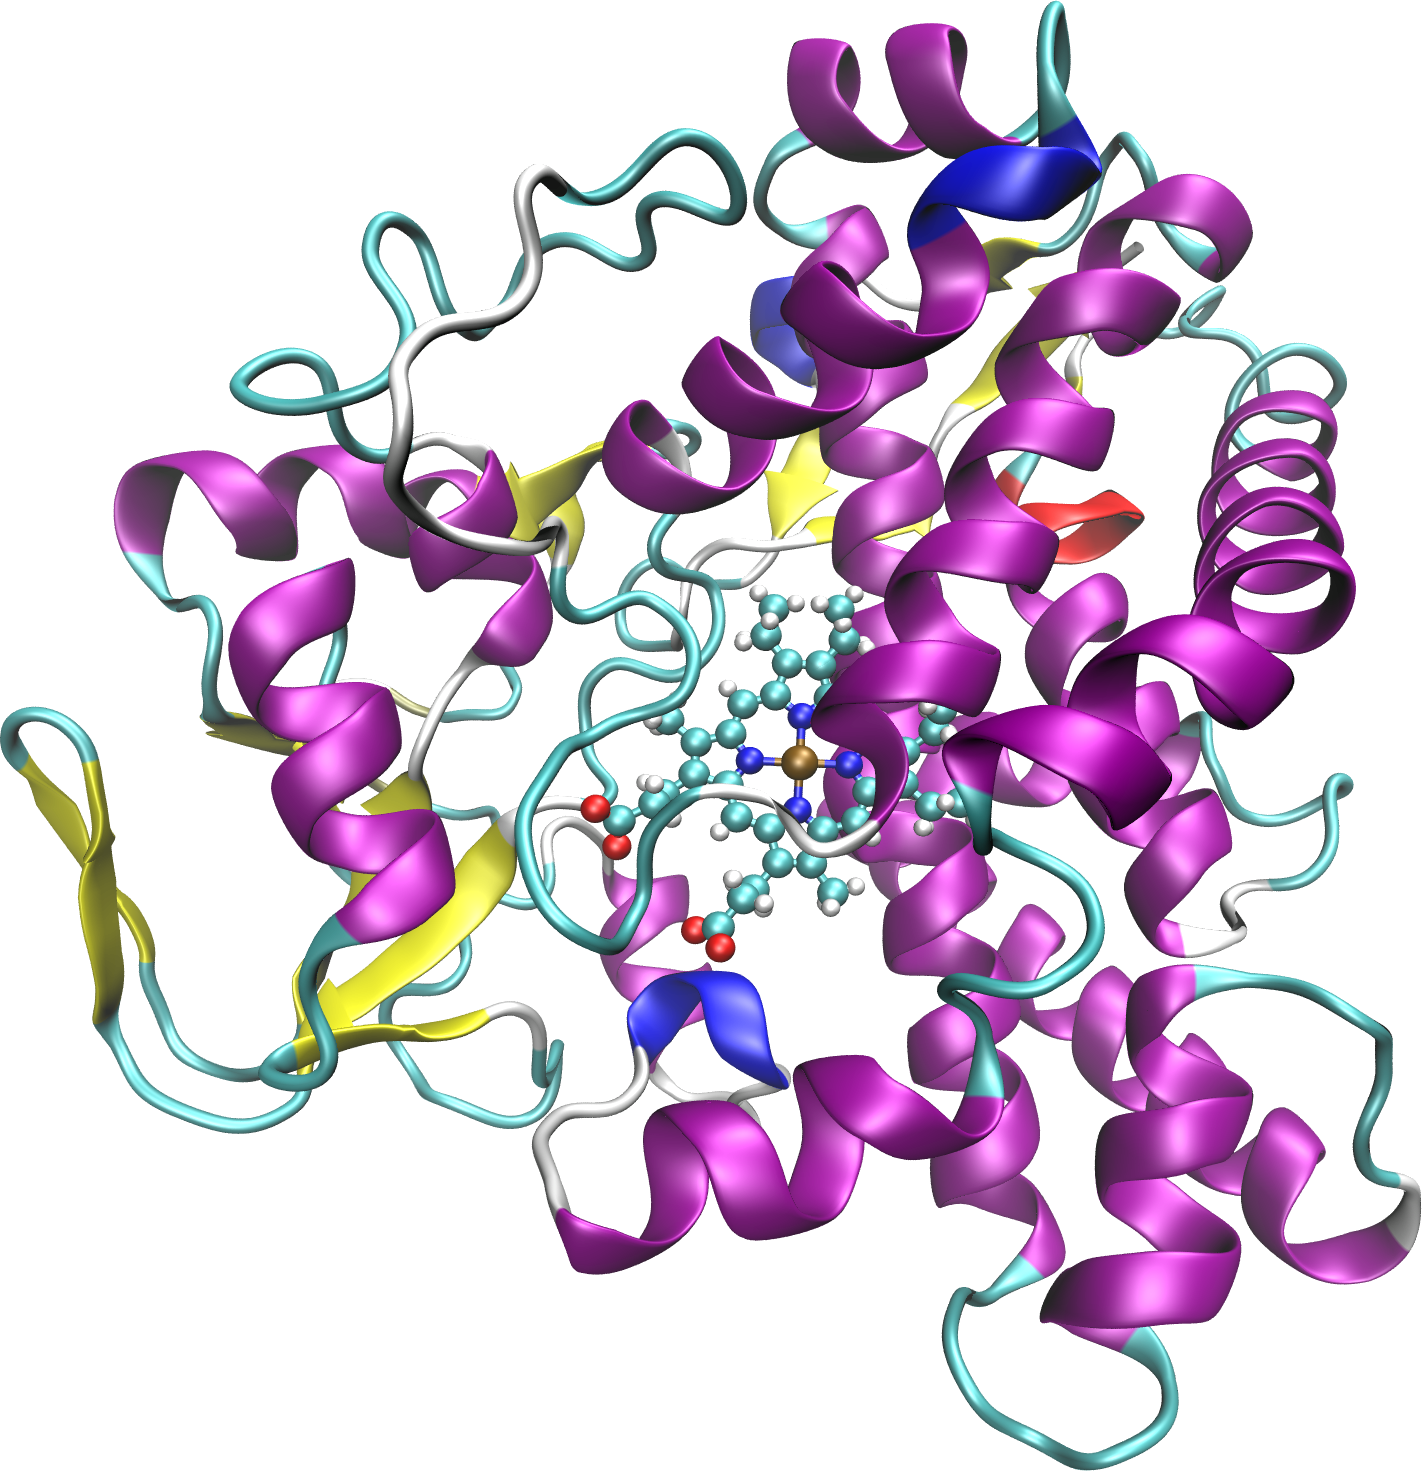
\includegraphics[width=0.5\textwidth]{figures/p450.png}
\caption{
The structure of cytochrome P450, taken from PDBid 1JFB, shown in cartoon representation.
The bonded heme group, shown as ball and stick model, is visible in the center.
The brown iron atom is chelated by four deep blue nitrogen atoms. 
}
\label{fig:p450}
\end{figure}
Cytochrome p450 is critical to drug metabolism, being active in approximately 75\% of drugs which are cleared in this method \cite{guengerich2007cytochrome}. 
As covered in \ref{subsubsection:lead_optimization}, accurately predicting  absorption, distribution, metabolism, and excretion, characteristics of drug compounds can be a critical determining factor in determining drug efficacy, performance in clinical development stages, and the overall costs of bringing new drugs to market.
Because of the ubiquity of P450 in metabolic reactions of drugs, there is no other single enzyme family as significant to determining ADME as P450.   

The general form of the reaction most frequently catalyzed by P450 is 
\begin{equation}
\mathrm{RH + O_{2} + NADPH + H^{+}> → ROH + H_{2}O + NADP^{+}}
\end{equation}


The specific locations of sites of metabolism (SOM) on small molecules can have a profound effect on the ADME characteristics of a small molecule.
Some cancer drugs such as epipodophyllotoxins, ifosphamide, tamoxifen, taxol and vinca alkaloids, are converted into their active states by oxygenation at specific locations by P450 \cite{kivisto1995role}.
P450 is the body's primary defense against toxicity, usually catalyzing the conversion of toxic compounds into harmless products \cite{gonzalez2005role,guengerich2001common}.
However in certain cases, such as acetaminophen, it is possible for P450 to convert a harmless reactant into a toxic product \cite{chen1998oxidation}.


